% % % % % % % % % % % % % % % % % % % % % % % % % % % % % % % %
% import configuration
% % % % % % % % % % % % % % % % % % % % % % % % % % % % % % % %

% % % % % % % % % % % % % % % % % % % % % % % % % % % % % % % %
% Konfiguration
% % % % % % % % % % % % % % % % % % % % % % % % % % % % % % % %
\newcommand{\titleinfo}{Requirements Specification}
\newcommand{\subjectinfo}{Wireless Parachute Reefing System for Sounding Rockets}
\newcommand{\authorinfo}{Luca Jost}
\newcommand{\versioninfo}{0.1}
\newcommand{\docNr}{BA Reefing}
\newcommand{\dateinfo}{\today}

% Notes for SRS completion, uncomment the following command to suppress this output
\newcommand{\note}[1]{%
    \vspace{0.25cm}%
    \colorbox{grey}{%
        \parbox{\linewidth-6pt}{%
            \vspace{0.5cm}%
            \centering%
            \parbox{\linewidth-1cm}{%
                \footnotesize{#1}%
            }%
            \vspace{0.5cm}%
        }%
    }%
    \vspace{0.25cm}}
%\newcommand{\note}[1]{}

% % % % % % % % % % % % % % % % % % % % % % % % % % % % % % % %
% Packages, Layout, Units, etc.
% % % % % % % % % % % % % % % % % % % % % % % % % % % % % % % %
%%%%%%%%%%%%%%%%%%%%%%%%%%%%%%%%%%%%%%%%%%
% Dokument
%%%%%%%%%%%%%%%%%%%%%%%%%%%%%%%%%%%%%%%%%%
% Geometrie
\newcommand{\paperFormat}{a4paper}
\newcommand{\lPageMargin}{25mm}
\newcommand{\rPageMargin}{20mm}
\newcommand{\tPageMargin}{20mm}
\newcommand{\bPageMargin}{20mm}

\documentclass[11pt,oneside]{scrartcl}

\newcommand{\newpar}{\par\par}

\usepackage[pdftitle={\titleinfo},%
			pdfauthor={\authorinfo},%
			pdfcreator={pdfLatex, LaTeX with hyperref},
			pdfsubject={\subjectinfo},
			plainpages=false,
			pdfpagelabels,
			colorlinks,
			linkcolor=black,
			filecolor=black,
			citecolor=black,
			urlcolor=black]{hyperref}
			
\usepackage[scaled]{helvet}
%\renewcommand\familydefault{\sfdefault} 


% Headings
\usepackage{scrlayer-scrpage}

%%%%%%%%%%%%%%%%%%%%%%%%%%%%%%%%%%%%%%%%%%
% Package's
%%%%%%%%%%%%%%%%%%%%%%%%%%%%%%%%%%%%%%%%%%
\usepackage[acronym]{glossaries}

\usepackage[OT1]{fontenc}

\usepackage[utf8]{inputenc}

\usepackage[free-standing-units=true,use-xspace=true]{siunitx}

\usepackage{layout}
\setlength{\parindent}{0em}

\renewcommand{\baselinestretch}{1.2}
\renewcommand{\arraystretch}{1}
\newcolumntype{P}[1]{>{\centering\arraybackslash}p{#1}}

%% This changes default fonts for both text and math mode to use Herman Zapfs
%% excellent Palatino font.  Do not change this.
%\usepackage[sc]{mathpazo}

%% The AMS-LaTeX extensions for mathematical typesetting.  Do not
%% remove.
\usepackage{amsmath,amssymb,amsfonts,mathrsfs}

\usepackage[capitalize, noabbrev]{cleveref}	%cref starts with capital letter
\usepackage[usenames,dvipsnames]{pstricks}
\usepackage{setspace}
\usepackage{epsfig}
\usepackage{pst-pdf}
\usepackage{pst-all}
\usepackage{pstricks-add}
\usepackage{supertabular}
\usepackage[font=small,labelfont=bf]{caption}
\usepackage[font=footnotesize]{subfig}
\usepackage{footnote}
\usepackage{float}
\usepackage{multirow}
\usepackage{pdfpages}
\usepackage{pgf,tikz}
\usepackage{color}
\usepackage{titletoc}

\usepackage[makeroom]{cancel}
\usepackage{array}
\usepackage{trfsigns}
\usepackage{textcomp}
\usepackage{booktabs}
\usepackage{rotating}

\usepackage{listings}

\usepackage{tabto}
\renewcommand{\captionfont}{\scriptsize\slshape}

%Inhaltsverzeichnis
\setcounter{secnumdepth}{4}
\setcounter{tocdepth}{2}

%Geometrie
\usepackage[\paperFormat,left=\lPageMargin,right=\rPageMargin,top=\tPageMargin,bottom=\bPageMargin,includeheadfoot]{geometry}

\usepackage{lipsum}%dummy text only
\usepackage{tikz}
\usetikzlibrary{fadings}
\newcommand{\gradient}{\noindent%
    \begin{tikzpicture}
    \fill[black,path fading=west] (-0.5\linewidth,0) rectangle (0,0.1ex);
    \fill[black,path fading=east] (0,0) rectangle (0.5\linewidth,0.1ex);
    \end{tikzpicture}%
}

%%%%%%%%%%%%%%%%%%%%%%%%%%%%%%%%%%%%%%%%%%%%%%%%%%%%%%%%%%%%%%%%
% Environment Numbering
%%%%%%%%%%%%%%%%%%%%%%%%%%%%%%%%%%%%%%%%%%%%%%%%%%%%%%%%%%%%%%%%

%Abbildungsnumerierung anhand Kapitel
\renewcommand{\thefigure}{\arabic{section}.\arabic{figure}}
\makeatletter \@addtoreset{figure}{section} \makeatother

%Gleichungen anhand Kapitel
\AtBeginDocument{\numberwithin{equation}{section}}
\AtBeginDocument{\numberwithin{figure}{section}}
\AtBeginDocument{\numberwithin{table}{section}}


%%%%%%%%%%%%%%%%%%%%%%%%%%%%%%%%%%%%%%%%%%%%%%%%%%%%%%%%%%%%%%%%
% Farben
%%%%%%%%%%%%%%%%%%%%%%%%%%%%%%%%%%%%%%%%%%%%%%%%%%%%%%%%%%%%%%%%
\definecolor{black}{rgb}{0,0,0}
\definecolor{red}{rgb}{1,0,0}
\definecolor{white}{rgb}{1,1,1}
\definecolor{grey}{rgb}{0.8,0.8,0.8}
\definecolor{bgGray}{rgb}{0.95,0.95,0.95}
\definecolor{stringColor}{rgb}{0.16,0.00,1.00}
\definecolor{annotationColor}{rgb}{0.39,0.39,0.39}
\definecolor{keywordColor}{rgb}{0.50,0.00,0.33}
\definecolor{commentColor}{rgb}{0.25,0.50,0.37}

%%%%%%%%%%%%%%%%%%%%%%%%%%%%%%%%%%%%%%%%%%%%%%%%%%%%%%%%%%%%%%%%
% Listing Styles
%%%%%%%%%%%%%%%%%%%%%%%%%%%%%%%%%%%%%%%%%%%%%%%%%%%%%%%%%%%%%%%%
\lstdefinestyle{bash}{
  language=bash,
  basicstyle=\normalsize\ttfamily,
  backgroundcolor = \color{bgGray},
  xleftmargin = 0cm,
  xrightmargin = 0cm,
  framexleftmargin = 0em,
  frame=tb,
  showstringspaces=false
}

\lstdefinestyle{cpp}{
		%linebackgroundcolor={\ifodd\value{lstnumber}\color{bgGray}\else\color{white}\fi},   % choose the background color; you must add \usepackage{color} or \usepackage{xcolor}; should come as last argument
	backgroundcolor=\color{bgGray},
	basicstyle=\normalsize\ttfamily,        % the size of the fonts that are used for the code
	breakatwhitespace=false,         % sets if automatic breaks should only happen at whitespace
	breaklines=true,                 % sets automatic line breaking
	captionpos=b,                    % sets the caption-position to bottom
	commentstyle=\color{commentColor},    % comment style
	deletekeywords={...},            % if you want to delete keywords from the given language
	escapeinside={\%*}{*)},          % if you want to add LaTeX within your code
	extendedchars=true,              % lets you use non-ASCII characters; for 8-bits encodings only, does not work with UTF-8
	frame=tb,	                  	 % adds a frame around the code
	keepspaces=true,                 % keeps spaces in text, useful for keeping indentation of code (possibly needs columns=flexible)
	keywordstyle=\color{keywordColor}\bfseries,   % keyword style
	language=C++,                    % the language of the code
	morekeywords={*,...},            % if you want to add more keywords to the set
	numbers=none,                    % where to put the line-numbers; possible values are (none, left, right)
	numbersep=3pt,                   % how far the line-numbers are from the code
	numberstyle=\footnotesize\color{codeGray}, % the style that is used for the line-numbers
	rulecolor=\color{black},         % if not set, the frame-color may be changed on line-breaks within not-black text (e.g. comments (green here))
	showspaces=false,                % show spaces everywhere adding particular underscores; it overrides 'showstringspaces'
	showstringspaces=false,          % underline spaces within strings only
	showtabs=false,                  % show tabs within strings adding particular underscores
	stringstyle=\color{stringColor},     % string literal style
	tabsize=2,	                   % sets default tabsize to 2 spaces
	title=\lstname                   % show the filename of files included with \lstinputlisting; also try caption instead of title}
}


%%%%%%%%%%%%%%%%%%%%%%%%%%%%%%%%%%%%%%%%%%%%%%%%%%%%%%%%%%%%%%%%
% Einheiten
%%%%%%%%%%%%%%%%%%%%%%%%%%%%%%%%%%%%%%%%%%%%%%%%%%%%%%%%%%%%%%%%
%\usepackage[Gray,squaren]{SIunits} %\gray befehl heisst nun \Gray und \square heisst nun \squaren
% replaced by \usepackage[free-standing-units=true,use-xspace=true]{siunitx} but at the beginning of the document

%Spannung
\DeclareMathOperator{\V}{\volt}
\DeclareMathOperator{\mV}{\milli \volt}
\DeclareMathOperator{\uV}{\micro \volt}

%Strom
\DeclareMathOperator{\A}{\ampere}
\DeclareMathOperator{\mA}{\milli \ampere}
\DeclareMathOperator{\uA}{\micro \ampere}
\DeclareMathOperator{\nA}{\nano \ampere}

%Zeit
\DeclareMathOperator{\s}{\second}
\DeclareMathOperator{\ms}{\milli \second}
\DeclareMathOperator{\us}{\micro \second}
\DeclareMathOperator{\ns}{\nano \second}

%Kapazitaet
\DeclareMathOperator{\mF}{\milli \farad}
\DeclareMathOperator{\uF}{\micro \farad}
\DeclareMathOperator{\nF}{\nano \farad}
\DeclareMathOperator{\pF}{\pico \farad}
\DeclareMathOperator{\fF}{\femto \farad}

%Induktivitaet
\DeclareMathOperator{\mH}{\milli \henry}
\DeclareMathOperator{\uH}{\micro \henry}
\DeclareMathOperator{\nH}{\nano \henry}

%Widerstand
\DeclareMathOperator{\MO}{\mega \ohm}
\DeclareMathOperator{\kO}{\kilo \ohm}
\DeclareMathOperator{\mO}{\milli \ohm}
\DeclareMathOperator{\Ohm}{\ohm}
%Strecke
\DeclareMathOperator{\km}{\kilo \meter}
\DeclareMathOperator{\cm}{\centi \meter}
\DeclareMathOperator{\mm}{\milli \meter}

%Frequenz
\DeclareMathOperator{\GHz}{\giga \hertz}
\DeclareMathOperator{\MHz}{\mega \hertz}
\DeclareMathOperator{\Hz}{\hertz}
\DeclareMathOperator{\kHz}{\kilo \hertz}
\DeclareMathOperator{\mHz}{\milli \hertz}

%Leistung
\DeclareMathOperator{\kW}{\kilo \watt}
\DeclareMathOperator{\mW}{\milli \watt}
\DeclareMathOperator{\uW}{\micro \watt}
\DeclareMathOperator{\W}{\watt}

%Kreisfrequenz
\DeclareMathOperator{\rpers}{\radianpersecond}

%DeziBel
\DeclareMathOperator{\dB}{\deci \bel}
\DeclareMathOperator{\dBm}{\deci \bel \milli}

%Bit
\DeclareMathOperator{\Bit}{\text{Bit}}
\DeclareMathOperator{\kBit}{\text{kBit}}
\DeclareMathOperator{\MBit}{\text{MBit}}
\DeclareMathOperator{\Byte}{\text{Byte}}
\DeclareMathOperator{\kByte}{\text{kByte}}
\DeclareMathOperator{\MByte}{\text{MByte}}
\DeclareMathOperator{\ppm}{\text{ppm}}

\makeglossaries

\newglossaryentry{stm32}
{
        name=STM32,
        description={Is a family of 32-bit microcontrollers based on the \acrshort{arm} Cortex-M processors}
}

\newacronym{arm}{ARM}{Advanced \acrshort{risc} Machines}
\newacronym{risc}{RISC}{Reduced Instruction Set Computer}
\newacronym{nac}{NAC}{Network Access Control}
\newacronym{iot}{IoT}{Internet of Things}
\newacronym{fms}{FMS}{Fleet Management System}
\newacronym{ip}{IP}{Internet Protocol}
\newacronym{can}{CAN}{Controller Area Network}
\newacronym{usb}{USB}{Universal Serial Bus}
\newacronym{imu}{IMU}{Inertial Measurement Unit}
\newacronym{pcb}{PCB}{Printed Circuit Board}
\newacronym{soc}{SoC}{System on a Chip}
\newacronym{led}{LED}{Light-emitting Diode}
\newacronym{gnss}{GNSS}{Global Navigation Satellite System}
\newacronym{sae}{SAE}{Society of Automotive Engineers}







% % % % % % % % % % % % % % % % % % % % % % % % % % % % % % % %
% Dokument
% % % % % % % % % % % % % % % % % % % % % % % % % % % % % % % %
\begin{document}

% % % % % % % % % % % % % % % % % % % % % % % % % % % % % % % %
% Titelseite
% % % % % % % % % % % % % % % % % % % % % % % % % % % % % % % %
\newgeometry{left=20mm, right=20mm, top=10mm, bottom=10mm}

\hrule
\begin{minipage}{0.5\linewidth}
\begin{tikzpicture}[scale=1]
	\node[] at(0cm,0) {
\includegraphics[height=1.5cm,trim=0mm 0mm 0cm 0mm, clip]{images/ost_logo_de_rgb-eps-converted-to}};			
\end{tikzpicture}
\end{minipage}
%
\begin{minipage}[c][][b]{0.49\linewidth}
\begin{flushright}
	
\includegraphics[height=1.4cm]{images/aris-logo}
\end{flushright}
\end{minipage}
\hrule
\begin{center}
   	\vspace*{\stretch{1}}
   	\begin{flushright}
   		\sffamily
   		{\Huge\sffamily\bfseries\subjectinfo\par}
   		\par\noindent\rule[-1ex]{\linewidth}{2pt}\par
		\vspace{0.5cm}
   		\emph{\huge\sffamily\titleinfo}
   		\vspace{1cm}\par
   		{\large\sffamily\authorinfo}\\
   		\vspace{1cm}
   		{\sffamily Advisor: Prof. Andreas Breitenmoser}\\
   		{\sffamily Co-advisor ARIS: Jonas Binz}\\
    \end{flushright}
   	\vspace*{\stretch{2}}	
   	\newcolumntype{Y}{>{\setlength\hsize{0.2\hsize}\raggedright\arraybackslash}X}
   	\newcolumntype{Z}{>{\setlength\hsize{0.4\hsize}\raggedright\arraybackslash}X}
   	\renewcommand\arraystretch{1.5}
   	\sffamily
\end{center}
\cfoot{}
\vspace*{\stretch{0.5}}	
\hrule
{
    \footnotesize 
    \begin{flushright}
       %\sffamily\docNr\quad Version \versioninfo\linebreak
        \dateinfo
    \end{flushright}
}

\restoregeometry
	
% % % % % % % % % % % % % % % % % % % % % % % % % % % % % % % %
% Kopf und Fuszeile aktivieren
% % % % % % % % % % % % % % % % % % % % % % % % % % % % % % % %
\pagestyle{scrheadings}
\KOMAoption{headsepline}{true}
\KOMAoption{footsepline}{true}
\ihead{\footnotesize\normalfont\titleinfo}
%\chead{\footnotesize\normalfont\docNr}
\ohead{\footnotesize\normalfont\subjectinfo}
\cfoot{}
\setkomafont{pagenumber}{\normalfont}
\ofoot{\footnotesize\normalfont\dateinfo}
\cfoot{\footnotesize\normalfont\pagemark}
\ifoot{\footnotesize\normalfont\authorinfo}


% % % % % % % % % % % % % % % % % % % % % % % % % % % % % % % %
% Revision History
% % % % % % % % % % % % % % % % % % % % % % % % % % % % % % % %	
\contentsfinish
\clearpage

\newpage
	
% % % % % % % % % % % % % % % % % % % % % % % % % % % % % % % %
% Inhaltsverzeichnis
% % % % % % % % % % % % % % % % % % % % % % % % % % % % % % % %

%	{\linespread{1.0} \tableofcontents}
%	\newpage
	
% % % % % % % % % % % % % % % % % % % % % % % % % % % % % % % %
% Kapitel
% % % % % % % % % % % % % % % % % % % % % % % % % % % % % % % %
%	\newpage
%		
%	%damit " kein umlaut erzeugt und als Anführungszeichn verwendet werden kann
%	%\shorthandoff{"} %Abschalten mit\shorthandon{"}
%    
%    % Abbildungen
%    \listoffigures
%    \addcontentsline{toc}{section}{List of Figures}
%        
%    % Tabellen
%    \listoftables
%    \addcontentsline{toc}{section}{List of Tables}
%    
%    % Listings
%    \lstlistoflistings
%    \addcontentsline{toc}{section}{List of Listings}
%			
%	% Glossary and Acronyms
    \glsnogroupskiptrue
    \printglossary[type=\acronymtype]
    \printglossary
	\newpage
	
	%Includes
	\section{Introduction}
\label{sec:intro}

\subsection{Association}
The association Akademische Raumfahrt Initiative Schweiz (ARIS) brings together students from Swiss universities fascinated by space exploration. Formed around ETH Zurich, HSLU, ZHAW, UZH and OST the association engages it's members in engineering challenges by integrating theory and practice. ARIS is also offering a wide variety of Theses for parts and systems that can be integrated in their future rockets. 

\subsection{Background}
In order to reduce the drift of a sounding rocket's descent a multi stage recovery system is needed. Normally, at apogee, a drogue chute is deployed, and the main chute is released at a lower altitude. If a parachute inflates too rapidly it can cause extreme shock to the overall parachute system and rigging causing it to malfunction. In order to keep the loads to a minimum, the descent speed needs to be reduced but at the same time the rocket needs to come down to earth as fast as possible to reduce its drift. As the rockets developed by ARIS get bigger and heavier new methods need to be developed to reduce these loads.\newline
Reefing is something that prevents a parachute from opening too rapidly. With an active reefing system the main parachute can be deployed at apogee and slowly open at a low altitude. This would simplify and reduce the overall weight of the recovery system.
\medskip
\begin{figure}[h!]
	\centering
	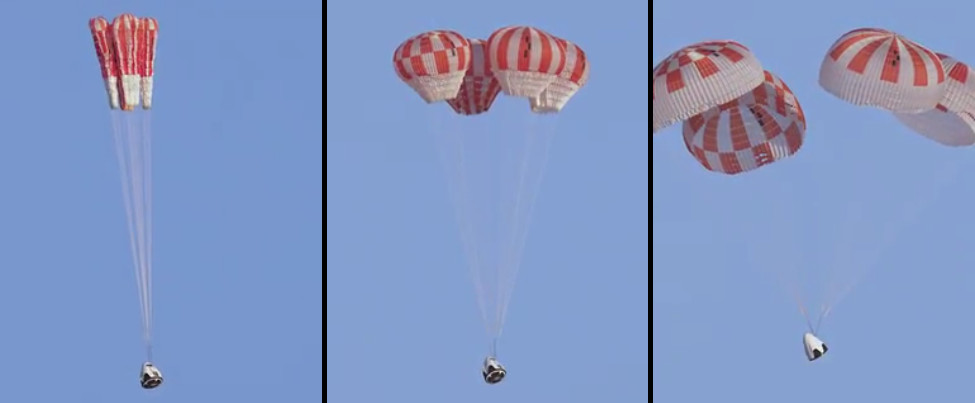
\includegraphics[height=6cm]{images/dragon.jpg}
	\caption{Dragon Reefing System}
	%\vspace{-2ex}
	%\caption*{\textbf{Source:} Original task definition}
	\label{fig:dragon_parachute}
\end{figure}

In the space industry reefing is often achieved by cutting lines inside the parachute. In the \cref{fig:dragon_parachute} above two lines are cut inside the parachute. This is often done by using pyrotechnic line cutters, activated by an electric signal.
	\section{Task Definition}

For this bachelor thesis methods for cutting a parachute line shall be investigated. A dedicated device has to be developed and manufactured to separate the parachute lines. The line cutter needs to be light and small enough to be placed inside the parachute as shown in Figure \ref{fig:cutter-placement}. Additionally the device needs to be durable to withstand forces acted on it during the deployment of the parachute.  

The line cutter interfaces through a wireless link, from the body of the rocket, with the main recovery computer. The computer can then initiate the separation of the reefing line. As a backup method, independent operation should also be supported. In that case, air pressure data shall be used to deploy the reefing line at a set altitude.

\begin{figure}[h!]
	\centering
	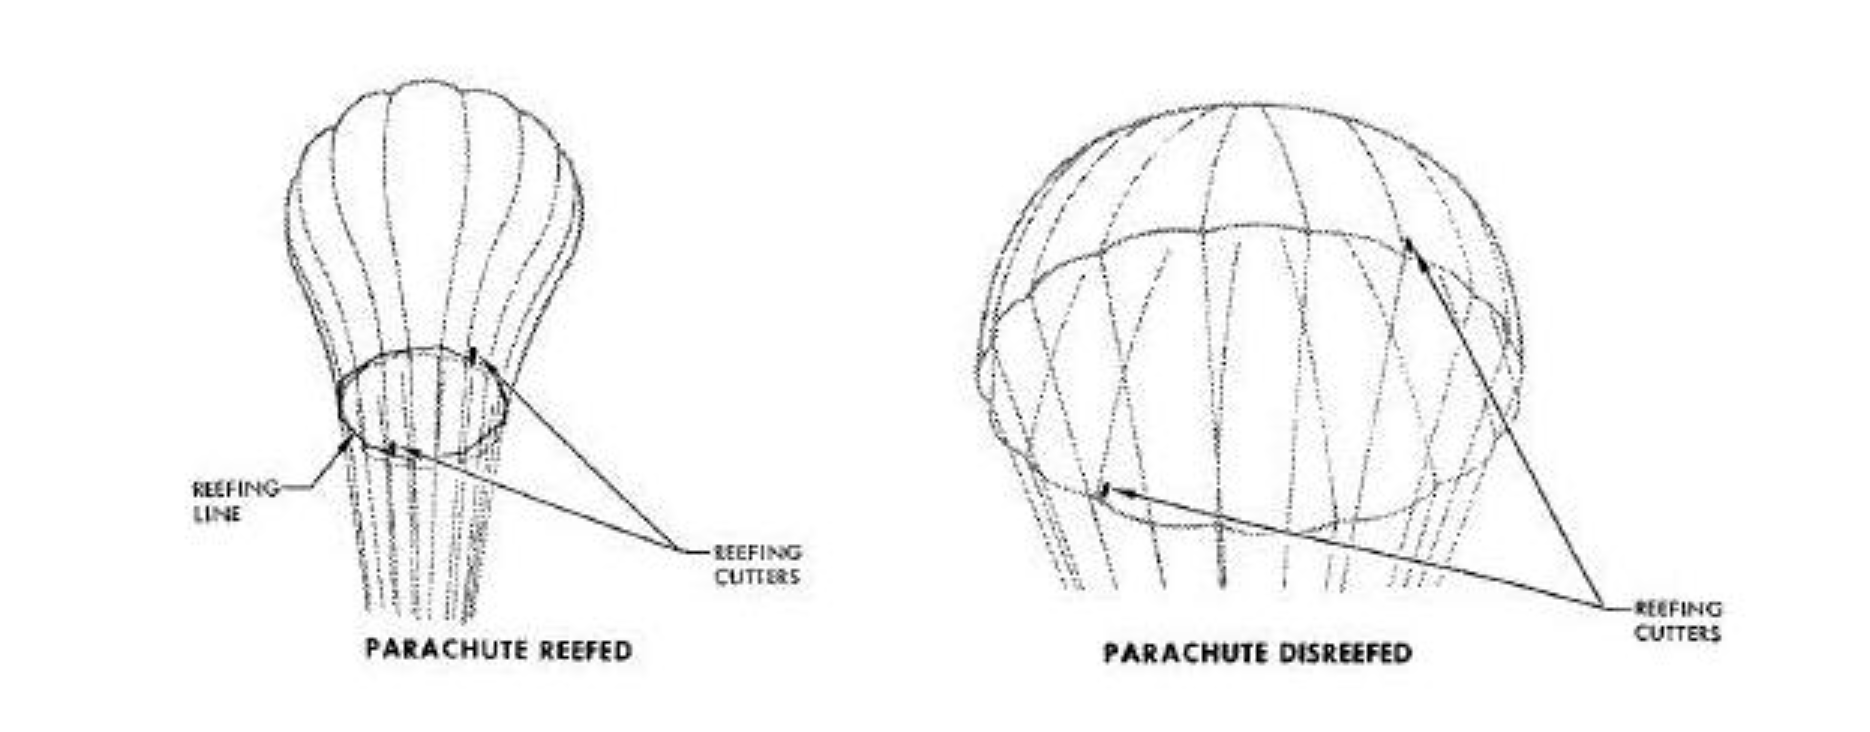
\includegraphics[height=7.3cm]{images/parachute_placement.png}
	\caption{Illustration of line cutter placement from NASA Gemini missions in 1963}
	%\vspace{-2ex}
	\label{fig:cutter-placement}
\end{figure}
	\newpage
\section{Product Requirements}

\subsection{Hardware}
The custom built hardware contains all necessary components integrated on a single \acrfull{pcb}. The hardware needs to comply with the following requirements: 
\begin{itemize}
		\item The hardware shall be based around an \gls{stm32} microcontroller.
		\item The hardware shall be able to do altitude measurements for independent operation.
		\item The hardware should use a wireless communication method to receive commands.
		\item The hardware should be able to do detect if the parachute was ejected (e.g. light sensor).
		\item The hardware shall be battery operated.
		\subitem The battery shall last at least 6 hours.
		\subitem A battery management system should be added to charge and monitor the battery.
		\item The hardware shall be enclosed in order to minimize dust and moisture getting into the system.
		\item The hardware shall weigh less than 150g
		\item The hardware shall have dimensions no bigger than 80x50x30mm
		\item The hardware shall be able to indicate the current device status (e.g. \acrshort{led}, buzzer).
		\item The hardware should have an \acrshort{usb} interface for configuration.
\end{itemize}
\medskip
\begin{figure}[h!]
	\centering
	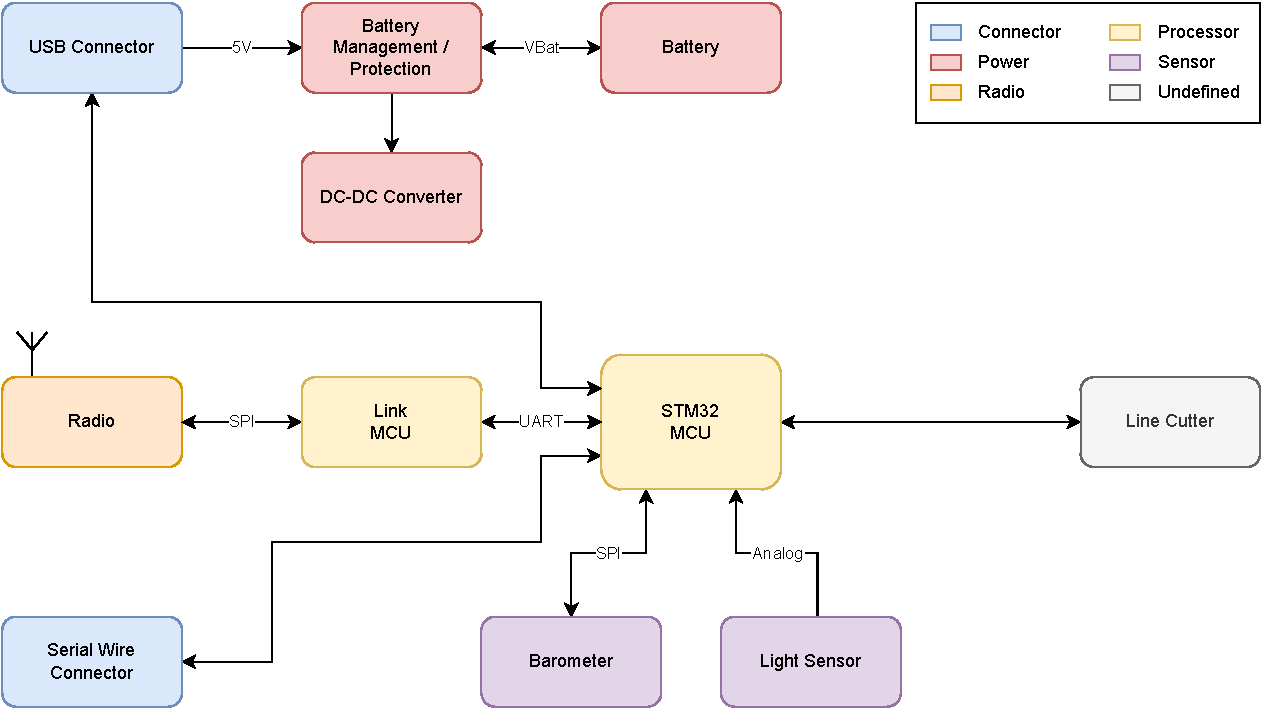
\includegraphics[height=7.3cm]{images/block_diagram}
	\caption{Example Hardware Block Diagram}
	%\vspace{-2ex}
	\label{fig:hardware_block_diagram}
\end{figure}

\newpage

\subsection{Line cutting mechanism}
The line cutting mechanism will be specifically developed for this application and needs to follow these requirements: 
\begin{itemize}
		\item The mechanism shall be able to separate the line in less than 10 seconds.
		\item The mechanism shall be reliable.
		\item The mechanism shall withstand forces acted on it during the deployment of the parachute

\end{itemize}


\label{sec:firmware}
\subsection{Firmware}
The embedded firmware will run on a \gls{stm32} and will be written in C. The requirements for the firmware are as follows:
\begin{itemize}
    \item The firmware shall connect to the transmitter.
    \item The firmware shall initiate the separation when commanded to.
    \item The firmware shall read air pressure data.
    \item The firmware shall be able to initiate the separation at a set altitude without a telemetry link.
    \item The firmware shall display the current device status to the user.
    \item The firmware shall offer an interface to configure the device through \acrshort{usb}.
\end{itemize}

	\input{sections/4_project_schedule}
	

% % % % % % % % % % % % % % % % % % % % % % % % % % % % % % % %
% ANHANG
% % % % % % % % % % % % % % % % % % % % % % % % % % % % % % % %
\appendix


%Nummerierung wieder auf roemisch umschalten

%\newpage
%\section{References}
%\label{anx:ref}
%% Do not repeat items covered in other documents or in a global project definitions and acronyms document
%\renewcommand{\refname}{} %kein Titel vor Literaturverzeichnis
%\vspace{-1.2cm}
%\bibliographystyle{ieeetr} %Literatur durchnumerieren
%\bibliography{lit}
%\nocite{*} %Alle Literatur aufführen
	
\end{document}